\section{Decay Angles}
\label{sec:decang}

In the next section we are interested in examining the distribution of the decay
angle between product pairs in various simulated decays. By examining the
distribution of decay angles in the laboratory frame this angle can be used to
distinguish the background (which should not have a strongly peaked angle
dependence) from the decays in which we are interested. This is due to the
ultra-relativistic parent particle beaming the decay products in the direction
of movement, while the background should not follow such a strongly beamed angle
distribution.

The decay angles were obtained by relativistically boosting the MC simulated
Lorentz vectors using the
\href{http://root.cern.ch/root/html/TLorentzVector.html\#TLorentzVector:Boost@1}{\texttt{Boost()::TLorentzVector}}
method.  The
\href{http://root.cern.ch/root/html/TVector3.html}{\texttt{TVector3}} vectors
used to boost the parent particles were obtained from fits to the momentum
component distributions of previously calculated LHCb MC simulation data. The
\href{http://root.cern.ch/root/html/TF1.html\#TF1:GetRandom}{\texttt{GetRandom()::TF1}}
method was then used to provide a random distribution following that of the
LHCb MC data. The boost was repeated a large number ($10^6$) of times, each
time boosted by a different 3-vector provided by the random momentum
distribution following the LHCb MC data, and each time the angle between the
resulting particles was calculated and plotted to provide final angle
distribution functions in the lab frame. This angle distribution can then be
used to distinguish these vital decays from the background, provided it is
sharply peaked enough.

\subsection{$\psi(3770) \rightarrow D^0 \xbar{D^0}$ decay}
\label{sec:decang-psidecay}

The first decay for which this was done was the $\psi(3770) \rightarrow D^0
\xbar{D^0}$ decay.

Before the LHCb MC momentum component distribution data could individually be
used to provide 3-vectors to boost the $\psi(3770)$, it had to be established
that there was no correspondence or correlation between the individual momentum
components. Table \ref{tab:psi-correlation-factors} shows the calculated
correlation factors between the individual direction components, whilst Figure
\ref{fig:psi-correlation-graphs} visualises the dependence of the components on
one another. Both clearly show no correlation between individual momentum
components. Thus, they can be considered independent distributions and the
random component generation can be done separately.

\begin{center}
\begin{table}
  \begin{tabu}{| c |[1.25pt] c | c | c |}
    \hline
    & \LARGE $p_x$ & \LARGE $p_y$ & \LARGE $p_z$ \\
    \tabucline[1.25pt]{-}
    \LARGE $p_x$ & 1 &  0.00640212 & 0.0150375 \\
    \hline
    \LARGE $p_y$ & 0.00640212 & 1 & 0.0167604 \\
    \hline
    \LARGE $p_z$ & 0.0150375 & 0.0167604 & 1 \\
    \hline
  \end{tabu}
  \label{tab:psi-correlation-factors}
\end{table}
\end{center}


\begin{center}
    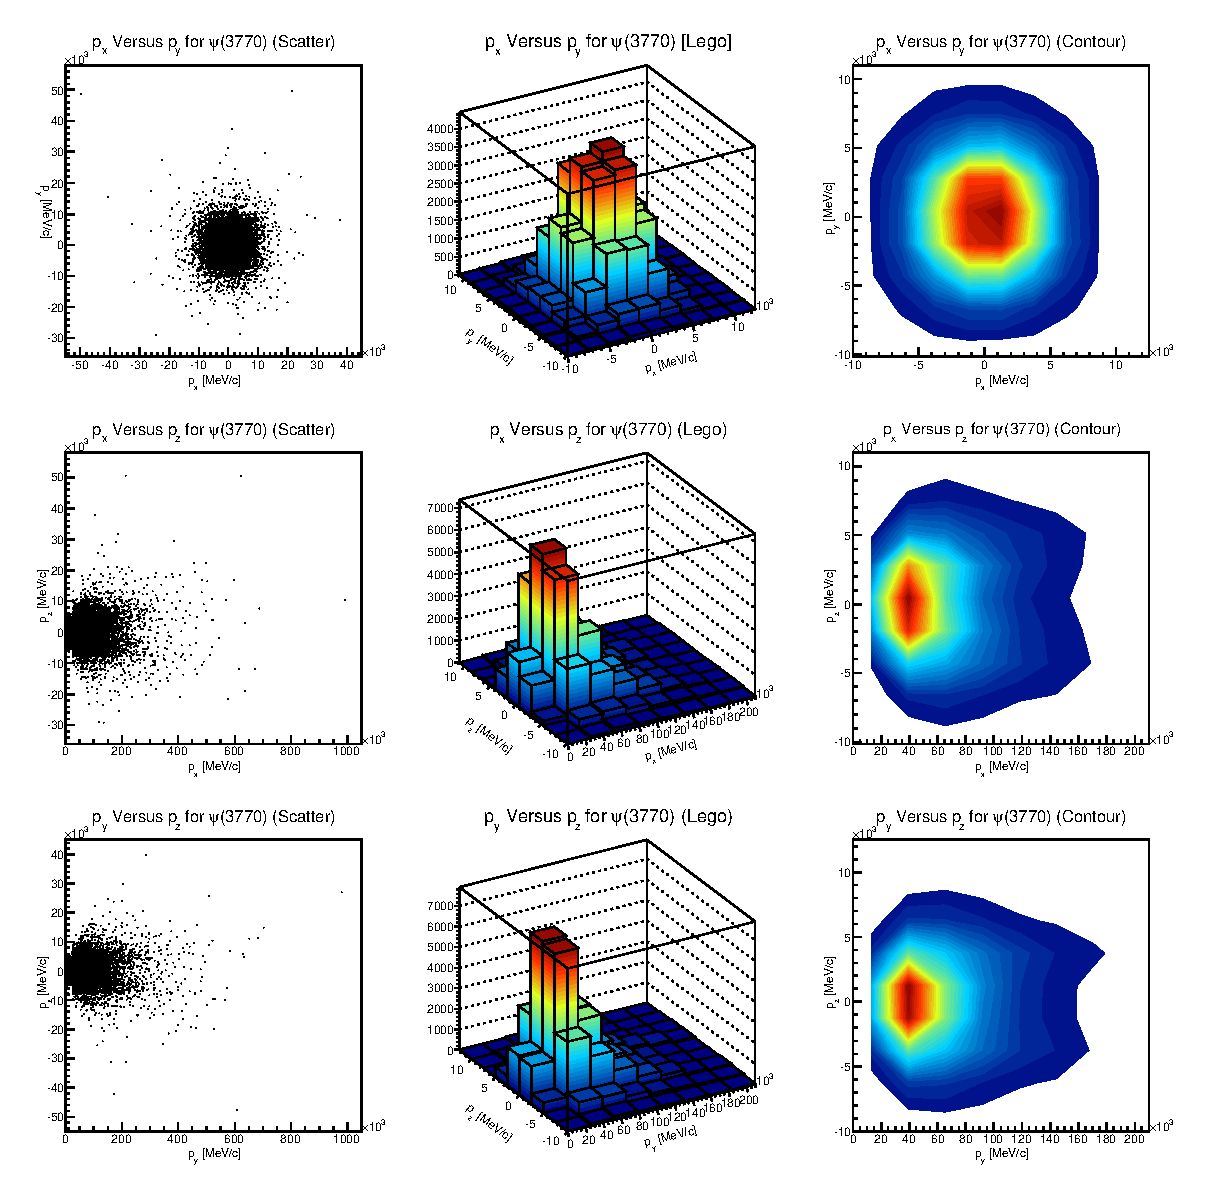
\includegraphics[width=\linewidth]{graphs/PsiMomentumComponentCorrelation.eps}
    \captionof{figure}{Different visualisations of the correlation between
        different momentum components in the LHCb MC data. These clearly show no
        correlation. Note that the $x-z$ and $y-z$ plots are skewed to the right
        as $z$ is always positive.}
    \label{fig:psi-correlation-graphs}
\end{center}

The $x$ and $y$ components of the momentum were fitted to Gaussian
distributions, whilst the $z$ component of the momentum was fitted to a Landau
up until \SI{62}{\giga\electronvolt\per\c}, after which it was fitted to a
Gaussian, as shown in Figure \ref{fig:psi-components}. Note that the fits are
not perfect, but follow the general distribution satisfactorily for the purposes
of our random momentum generation.

\begin{center}
    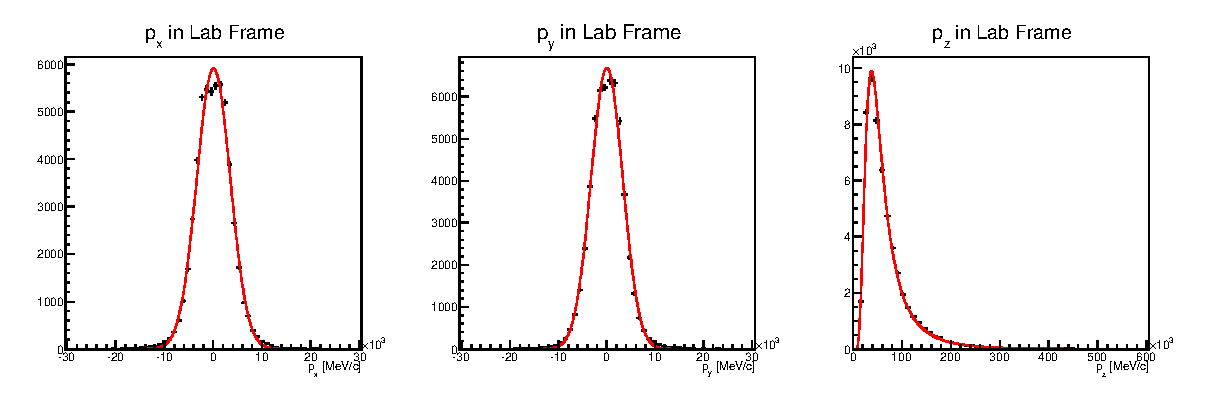
\includegraphics[width=\linewidth]{graphs/PsiMomentumComponentFit.eps}
    \captionof{figure}{Fits to the momentum component distributions.
        \texttt{ROOT}'s \texttt{GetRandom()::TF1} method was then used to provide a
        random distribution based on these fits.}
    \label{fig:psi-components}
\end{center}

The final decay angle distribution between the $D^0$ and $\xbar{D^0}$ is shown
in Figure \ref{fig:psi-angle}. Note that all decay angles are $< 5\degree$,
with a high peak at around $\sim 0.5\degree$, meaning that the decay angle
can be used to separate the $\psi(3770)$ decays from the background.

\begin{center}
    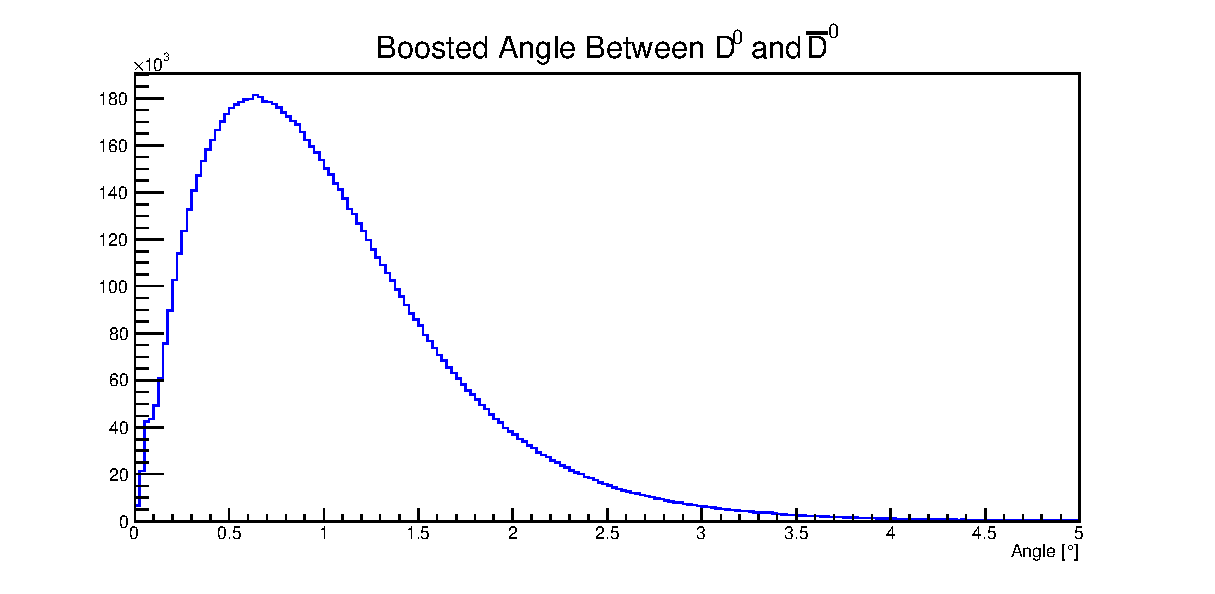
\includegraphics[width=\linewidth]{graphs/PsiBoostedAngle.eps}
    \captionof{figure}{The final lab frame decay angle distribution between
        $D^0$ and $\xbar{D^0}$. Note that the distribution is sharply peaked
        about $\sim 5\degree$, with no angles $> 5\degree$.}
    \label{fig:psi-angle}
\end{center}

\subsection{$B \rightarrow (\psi(3770) \rightarrow D^0 \xbar{D^0})K$ decay}
\label{sec:decang-bdecay}

As with the $\psi(3770)$ decay, LHCb MC momentum data was used to provide a
distribution to use for the Lorentz boost. However, only $B \rightarrow D~Bach$
(where the bachelor particle is either a kaon or a pion) momentum data was
available. Hence conservation of momentum was used to determine the parent $B$
momentum from the $D$ and bachelor particle momenta.

The corresponding correlation factor table is shown below in Table
\ref{tab:b-correlation-factors}, while the correlation visualisations are shown
in Figure \ref{fig:b-correlation-graphs}:

\begin{center}
\begin{table}
  \begin{tabu}{| c |[1.25pt] c | c | c |}
    \hline
    & \LARGE $p_x$ & \LARGE $p_y$ & \LARGE $p_z$ \\
    \tabucline[1.25pt]{-}
    \LARGE $p_x$ & 1 &  0.0165178 & -0.00486466 \\
    \hline
    \LARGE $p_y$ & 0.0165178 & 1 & 0.017408 \\
    \hline
    \LARGE $p_z$ & -0.00486466 & 0.017408 & 1 \\
    \hline
  \end{tabu}
  \label{tab:b-correlation-factors}
\end{table}
\end{center}


\begin{center}
    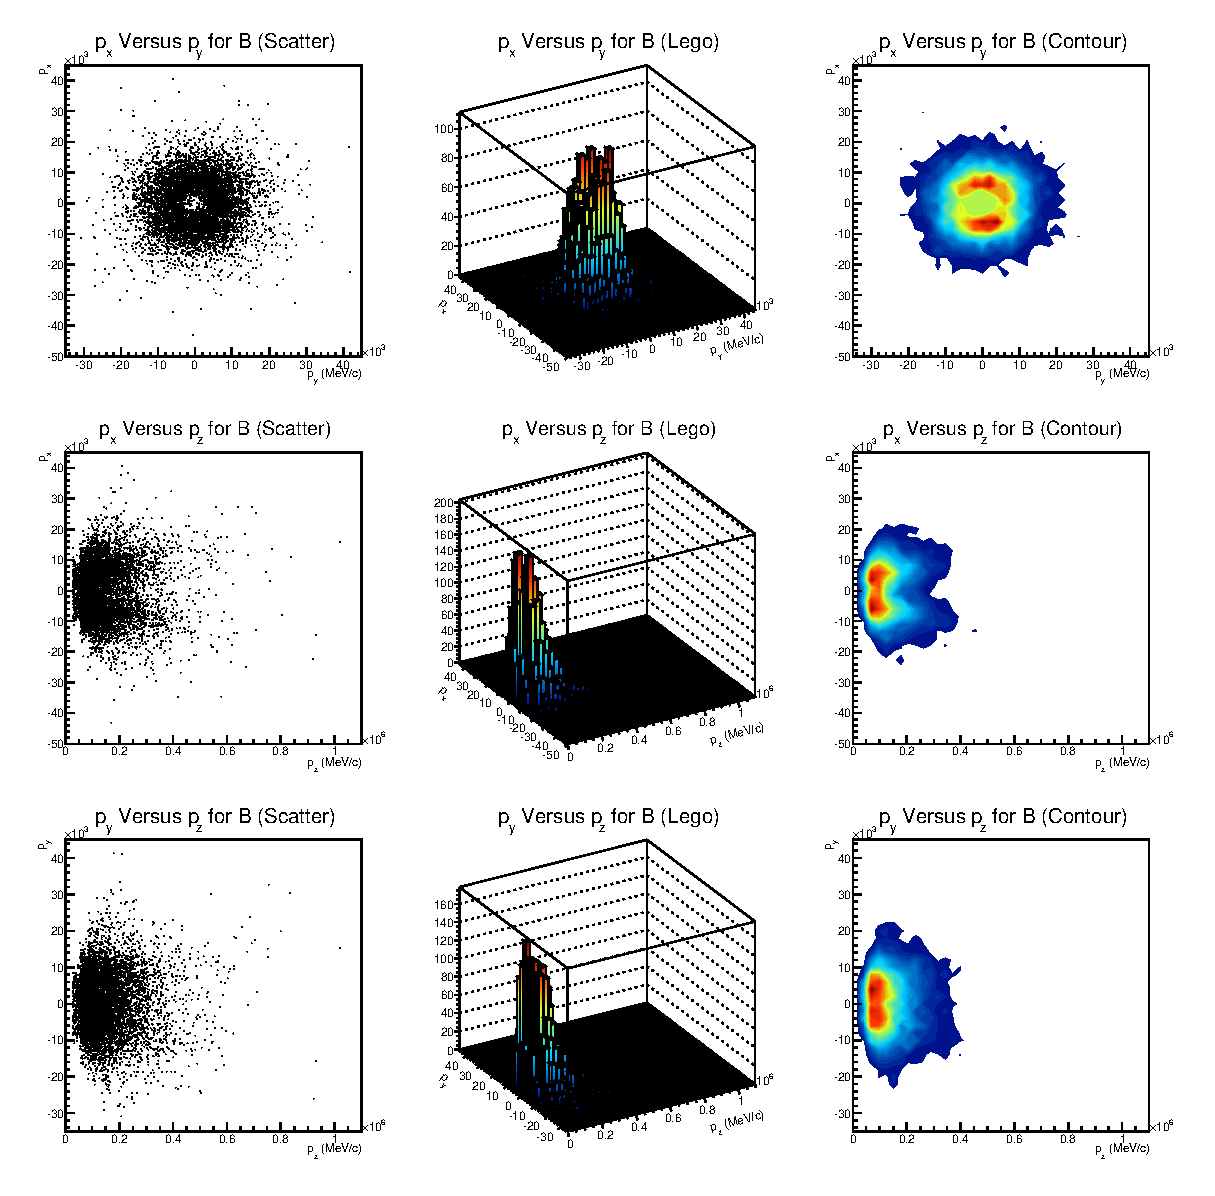
\includegraphics[width=\linewidth]{graphs/BMomentumComponentCorrelation.eps}
    \captionof{figure}{Visualisations of the correlation between momentum
        components of the $B$ meson, obtained from $B \rightarrow D~Bach$ LHCb
        MC data. Note the hole present in the $x-y$ graphs.}
    \label{fig:b-correlation-graphs}
\end{center}

The momentum components were once again fitted to mathematical functions, again
a Gaussian for $x$ and $y$ components and for the $z$ component a Landau up
until \SI{130}{\giga\electronvolt\per\c}, after which a Gaussian. Note that the
$x$ and to a lesser extent the $y$ component distributions cut off at low
values. This is most likely due to specific detector design and is thus ignored
for the purposes of the mathematical fit, which intends only to find the general
distribution of $B$ meson momentum components. The resulting fits are
illustrated in Figure \ref{fig:b-components}.

\begin{center}
    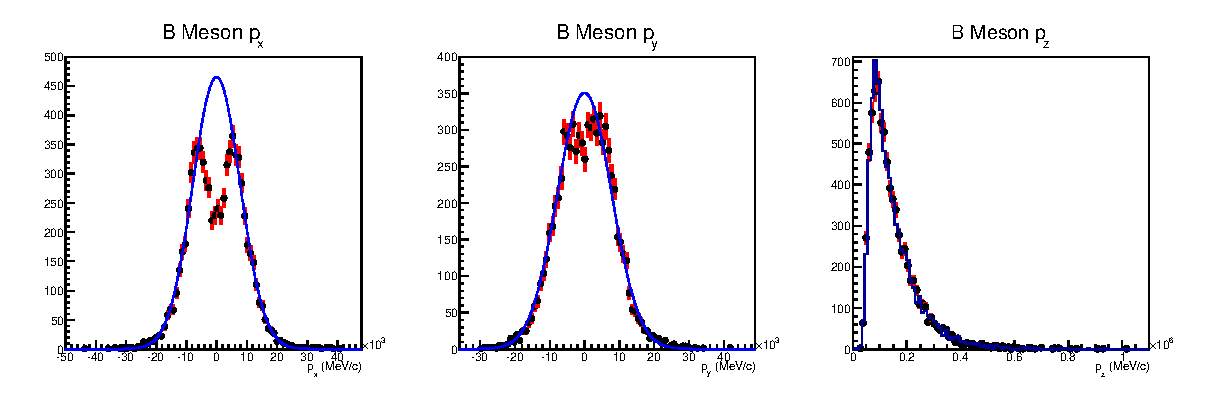
\includegraphics[width=\linewidth]{graphs/BMomentumComponentFit.eps}
    \captionof{figure}{The momentum component distributions for the $B$ meson,
        along with their mathematical fits. Note the gap in the $x$ and $y$
        component distributions near the $0$ point.}
    \label{fig:b-components}
\end{center}

The angle distributions between the $\psi(3770)$ and $K$ and between the $D^0$
and $\xbar{D^0}$ product particles was then plotted both in the rest frame of
the parent $B$ meson and in the lab frame, i.e. the Lorentz boosted frame. The
plots are shown below in Figures \ref{fig:b-non-boost-angle,fig:b-boost-angle}:

\begin{center}
    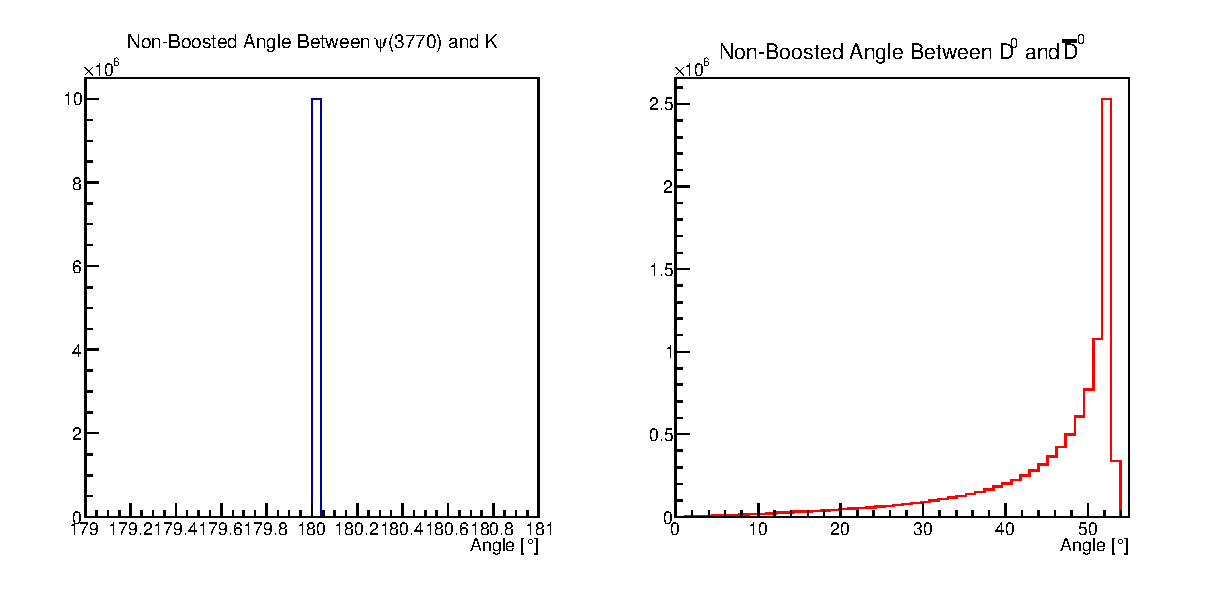
\includegraphics[width=\linewidth]{graphs/BMomentumNonBoostAngle.eps}
    \captionof{figure}{The decay angle distributions in the rest frame of the
        parent $B$ meson. Note the sharp cut off at $\sim 50 \degree$ for the
        $D^0$-$\xbar{D^0}$ decay angle distribution.}
    \label{fig:b-non-boost-angle}
\end{center}

\begin{center}
    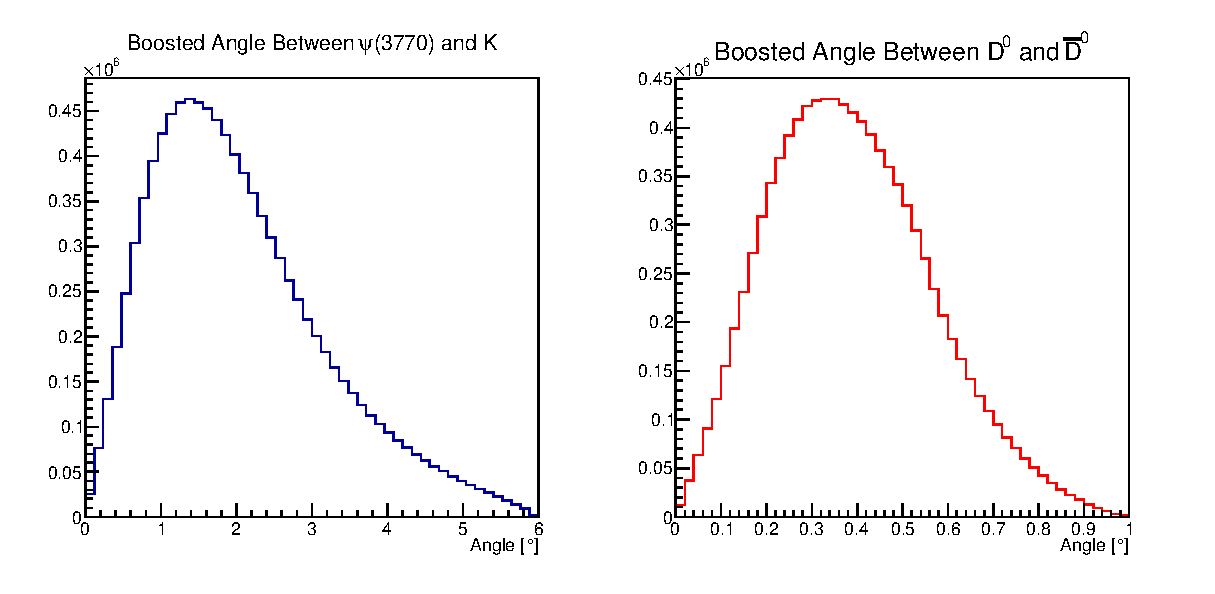
\includegraphics[width=\linewidth]{graphs/BMomentumBoostAngle.eps}
    \captionof{figure}{The decay angle distributions in the lab frame. Note that
        both distributions are contained within a small range of angles, $\lesssim 6
       \degree$ for the $\psi(3770)$-$K$ angle and $\lesssim 1 \degree$ for the
       $D^0$-$\xbar{D^0}$ angle.}
    \label{fig:b-boost-angle}
\end{center}

Both of these distributions are contained in a small range of
angles and are sharply peaked, with the $\psi(3770)$-$K$ angle at around $\simeq
1.5\degree$, and the $D^0$-$\xbar{D^0}$ angle at around $\simeq 0.4\degree$.
This confirms that $B \rightarrow (\psi(3770) \rightarrow D^0 \xbar{D^0}) K$
decays can be easily distinguished from the background due to the sharp angular
peaking in the $\psi(3770) \rightarrow D^0 \xbar{D^0}$ product decay, allowing
for its use in isolating $\psi(3770)$ decays for the study of symmetry
violation.
